\documentclass{acmsiggraph}

%% The 'helvet' and 'times' packages define the typefaces used for
%% serif and sans serif type in this document. Computer Modern Roman
%% is used for mathematics typesetting. The scale factor is set to .92
%% to bring the sans-serif type in line with the serif type.
\usepackage[scaled=.92]{helvet}
\usepackage{times}
\usepackage[utf8]{inputenc}
\usepackage[T1]{fontenc}

%% The 'graphicx' package allows for the inclusion of EPS figures.
\usepackage{graphicx}

%% use this for zero \parindent and non-zero \parskip, intelligently.
\usepackage{parskip}
\setlength{\itemsep}{0pt}

%% Optional: the 'caption' package provides a nicer-looking replacement
%% for the standard caption environment. With 'labelfont=bf,'textfont=it',
%% caption labels are bold and caption text is italic.
\usepackage[labelfont=bf,textfont=it]{caption}

%% Paper title.
\title{WebGL Massively Multiplayer Online Game}

%% Single author
%%\author{Roy G. Biv\thanks{e-mail: roy.g.biv@aol.com}\\Allied Widgets Research}

%% Multiple authors
\author{Student\\ Gianni Chen\\ giannic@seas.upenn.edu\\ University of Pennsylvania
\and Advisor\\ Professor Norm Badler\\ badler@seas.upenn.edu\\ University of Pennsylvania
\and Advisor\\ Aline Normoyle\\ alinen@seas.upenn.edu\\ University of Pennsylvania}

%% Keywords that describe your work.
\keywords{webgl, mmo, game, online}

%% Citation Reference
%% Citations can be done this way~\cite{Jobs95} or this more concise 
%% way~\shortcite{Jobs95}, depending upon the application.

%% Images
%% \begin{figure*}[ht]
%% \centering
%% \includegraphics[width=2.5in]{sample.eps}
%% \caption{Sample illustration.}
%% \end{figure*}

%%%%%% START OF THE PAPER %%%%%%
\begin{document}
\teaser{
    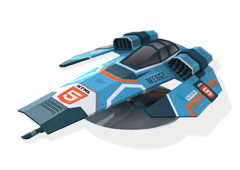
\includegraphics[width=2in]{hexmki.png}
    \caption{Hexmki, HexGL's main model}
}

%% The ``\maketitle'' command must be the first command after the
%% ``\begin{document}'' command. It prepares and prints the title block.
\maketitle

\begin{abstract}
\begin{itshape}
% The purpose of this document is three-fold. First, it describes the requirements of the project proposal. Second, it presents this information in a style your proposal should mimic. Third, it helps teach academic writing techniques. Your proposal is expected to have an abstract. An abstract is a two-paragraph maximum executive summary of your work. It should briefly outline your problem statement and its (expected) contributions.
% \\\\
We will build a multiplayer online game using WebGL and web sockets. Players will connect to a server in their browsers and be able to view other players who are also connected. The goal of each player is to eliminate the others in a free for all format. The players are ranked through the prescribed calculations involving eliminations, deaths, and other properties. This is a simplified combination of current approaches which are either solely WebGL demonstrations or HTML5 and web socket games. One of our primary goals is to provide a stepping stone to build more sophisticated multiplayer online WebGL games.
\\\\
Project Blog: http://webglmmo.blogspot.com
\end{itshape}
\end{abstract}

%% The ``\keywordlist'' command prints out the keywords.
%% \keywordlist

\hrulefill
\section{Introduction}

% You should begin by introducing your topic. In this section, you should define the core terminology specific to the field, introduce the problem statement, and make clear the benefits (motivate!) of resolving that problem statement. The main difference between the Abstract and Introduction sections is that the abstract summarizes the entire project, including results, whereas the introduction only provides the motivation of the problem and an overview of the proposed solution.
% \\
Since the late 1990s, Massively multiplayer online games (MMOG) have been a popular alternative to other games as well as a pleasant escape from everyday life. This was made possible not only by the improvements to our internet systems, but also by the increased power of our local machines. More recently, many classic games have been making reimagined appearances as MMOGs in our browsers. Common ways to achieve the real-time aspect include Comet, a model which allows pushing of data to a browser without request, and sockets, which has a variety of implementations on the web for asynchronous input and output. We have also seen a movement of 3D graphics towards the web, starting from Flash to Canvas 3D and in 2011, the first stable release of the Web Graphics Library (WebGL). While WebGL allows for both 2D and 3D rendering, the \emph{multiplayer} games we currently see are often in 2D. It is rare to see a multiplayer online game built in 3D using WebGL.
\\\\
In the initial time frame of this project, we will implement a barebone game. The motivation is not to build the next World of Warcraft, but to set a base for those who would like to build full-feature multiplayer WebGL games in the future. Though the code base will be presented as a game instead of a boilerplate, parts of it should be adaptable to new environments for their respective purposes. This will be helpful to the games community as well as related researchers because it can be used as a rapid prototyping tool. There are parallels that can be drawn between this project and tools such as Twitter Bootstrap for their base functionalities in different fields.
\\\\
Our project aims to combine the two very new technologies, WebGL and WebSocket, to build a very simple 3D MMOG. We will start by learning the technologies required for implementation. Once some familiarity is established, we will first implement an interactive 2D environment in WebGL for a local machine. Then, we will build upon that to make a 3D environment, bringing it a step closer to the desired look and feel. At this stage, we will begin to prototype some game features and dynamics. Then, we can begin experimenting with the WebSocket protocol on the 2D prototype to support multiple players. Once we successfully have multiplayer input, we will generalize it to the 3D environment to achieve our desired outcome.
\\\\
This project makes the following contributions:
\begin{itemize}
    \item{Explores a new alternative for gamers on the web}
    \item{Establishes a new front and back end combination for web games and developers who may be interested}
    \item{Provides base code for future WebGL multiplayer environments}
\end{itemize}

% Answer each of the following questions in one paragraph to compose your introduction: \\
% \textbf{Problem Statement} \\
% One paragraph to describe the problem that you are tackling. \\

% \textbf{Motivation} \\
% Why is this problem interesting and relevant to the (graphics/games/UI) research community? \\

% \textbf{Proposed Solution} \\
% How do we propose to tackle this problem (that has been identified in the previous paragraphs, is interesting to the community, and has yet to be tackled by other researchers)? \\

% \textbf{Contributions} \\
% An enumeration of the contributions of the senior design project\\
% This project makes the following contributions:
% \begin{itemize}
%     \item{Contribution 1}
%     \item{Contribution 2}
% \end{itemize}

    \subsection{Design Goals}
    % Who is the target Audience for your project? How does the audience benefit? What goals or objectives will you solve for the user?
    There are two major audiences for this project: casual online gamers and web game developers. The target consumer is any person who has access to the web and has an interest in interacting with others through games. This is a broad audience, but we have seen in the past that many people are fascinated by interactions as simple as seeing people in another continent through a camera in the shape of a telescope on the street (Appendix). We want users to feel a competitive connection with others who are in the same virtual space. On the other end of the spectrum, this framework will target game developers, especially those interested in web technologies. Like Twitter Bootstrap provides website developers a quick way to host content, this project will allow game developers a quick way to build a functional game.

    \subsection{Project Proposed Features and Functionality}
    This project implements the following features and functionality:
    \begin{itemize}
        \item{An interactive 3D environment accessible by anyone with a WebGL supported browser}
        \item{Support for multiple players to interact in the environment}
        \item{A way for players to navigate the environment}
        \item{A way for players to eliminate one another}
            \subitem{e.g. weapons, elements etc.}
        \item{A competitive way for players to avoid being eliminated}
            \subitem{e.g. jumping, shielding, etc.}
        \item{A presentable and deliverable open source base code}
    \end{itemize}

\section{Related Work}
% Perhaps the most important section of your proposal is related work. In this section, create a taxonomy of prior work relevant for your project. Here you demonstrate that you have read and understand what others in the field have done. This ensures you (1) know the state-of-the-art, (2) are not  directly copying others work, and (3) you know the performance levels you must achieve to make a contribution. As you discuss each related work, make note of how each has advanced the field. Then, enumerate how your project extends and enhances prior work.
Web games in the browser collectively have the largest user base. This reason has driven development for this particular medium for games to explode in the past two years. While the traditional tools used to build these were Java and Flash, more and more developers have chosen to move to HTML5 due to its advantages in efficiency and compatibility. More recently, with the release of WebGL, some developers have experimented with it in conjunction with HTML5 for its advanced rendering capabilities. It is difficult to find official papers on this subject in graphics conferences, but there have been some presentations and courses. One such example that I will be using as a tool for learning this  technology is \emph{Introduction to WebGL}~\cite{J12}. Found across the web, we see a variety of projects from individual developers to larger organizations. We have described a few notable ones.

    \subsection{Khronos Group SIGGRAPH}
    The Khronos Group consists of media centric companies such as NVIDIA, Electronic Arts, and Google, among others. They focus on creating "open standard, royalty-free APIs" which allow graphics developers to create content for interested users or consumers. At SIGGRAPH, they have a variety of presentations on these standards and libraries, including tutorials which give an overview of their current capabilities. For example, at SIGGRAPH 2012, they presented \emph{Graphics Programming for the Web: WebGL}~\cite{RM12}.

    \subsection{Chrome Experiments}
    Chrome Experiments, hosted by Google, is a collection of some of the most creative web experiments using cutting edge web technologies such as HTML5 and WebGL. They demonstrate just how powerful these tools are and provide a point of references for state-of-the-art web technologies. Many developers have built their applications with this collection as a driving force for improvement. Many of these submissions have are open source and provide a useful means of learning the standards, conventions, and techniques in developing with these tools. For instance, in the projects tagged multiplayer, DCubic has implemented a space where multiple users can connect and create cubes in space of various colors and animation features~\cite{P12}.

    \subsection{BrowserQuest}
    BrowserQuest is a MMORPG adventure game built by Mozilla Foundation~\cite{AJK13} and Little Workshop. Little Workshop is a duo, Guillaume Lecollinet and Frank Lecollinet, based in Paris, France~\cite{LL12}. It is implemented using HTML5 Canvas and WebSockets. It is now an open source project hosted on Github. It was originally meant to be a demo of how these technologies can be used to implement a game, explaining why the in-game population has declined since. It hosts several load-balanced servers, with multiple environment in each one. Upon connection, the player can interact with other players in the environment they were connected to. Another notable contribution of BrowserQuest is its compatibility with mobile devices (iOS, Android, Firefox).

    \subsection{HexGL}
    HexGL is a HTML5 and WebGL game single player racing game built by Thibaut Despoulain, a senior Computer Engineering student at Université de technologie Belfort-Montbéliard. This too, had optimizations to bring the game to mobile. This impressive demo was one of the first noted to use three.js, a library built on top of WebGL. For that reason, it was later added as an entry to Chrome Experiments~\cite{D12}.

    % \subsection{Example Subsection Header}
    % This section should have in-line citations to your bibliography. We are going to require that your proposal has (at least) 6 references. List all bibliographical references in 9-point Times, single-spaced, at the end of your paper in alphabetical order. If you are using bibtex, compiling using the instructions in the README will ensure the references are included at the end.  When referenced in the text, enclose the citation index in square brackets, for example [Lou90] or ~\cite{Jobs95} if you are using the bibtex. Where appropriate, include the name(s) of editors of referenced books.\\

    % For references, please use the following format:
    % \begin{itemize}
        % \item{\textbf{one} author: first 3 characters plus year - e.g. [Lou90]}
        % \item{\textbf{two}, \textbf{three}, or \textbf{four} authors: first character of each family name plus year - e.g. [FH93] or [KSS97] or [LFTG97]}
        % \item{\textbf{more than 3} authors: first character of family name from first three authors followed by a '*' followed by the year - e.g. [BFH*98] or [FDF*93]}
    % \end{itemize}

\section{Project Proposal}
% Now is the time to introduce your proposed project in all of its glory. Admittedly, this will be difficult. Even so, setting and realizing realistic research goals is an important skill. Begin by summarizing what you are going to do and the expected benefit it will bring.\\
% PLEASE PROVIDE DETAILS IN THIS SECTION.
This project aims to create a functional 3-dimensional Massively Multiplayer Online Game. Its core components will be implemented with WebGL and the WebSockets protocol. We will first build a 3D environment. This will likely be a simple terrain, but is a means for interaction between multiple players. This space will be populated by users connecting from remote locations. Each user may be represented by something as simple as geometry moving in perspective space on keyboard input.
\\\\
The key here is that the users can interact with each other with minimal delay. To demonstrate this, the game will be a standard deathmatch, where any given player tries to eliminate as many other players as possible in order to climb the rankings. Upon elimination, a player will respawn in a random location. The means of attack for a player will be via a "shockwave" that radially emanates from the player itself in the horizontal plane. Other players can avoid elimination by jumping, that is changing their vertical height temporarily. This is a simple framework that will set a starting point for more sophisticated renderings of future MMOGs built with the same stack.

    \subsection{Anticipated Approach}
%    Having summarized what you are going to do, it’s time to describe how you plan to do it. Let us suppose you are going to create a service that takes a cell-phone picture of a building and returns the building’s name via text message. In this case you might want to talk about establishing a server to receive pictures via MMS. Once the picture is received, you will run an edge extraction algorithm over it. Then, similarity between the submitted picture and those stored (and tagged) in a MySQL database will be computing using algorithm XYZ. Finally, the tag of the most similar image will be returned to the user.
    The environment for this game will be in a finite space. We will define the terrain first with a simple rectangle, then import a terrain defined by an object file with changes in elevation at different points. This terrain will be the minimum $y$ value any player can be at. That is, it will be a rigid collision object.
    \\\\
    Suppose for now our players are represented by spheres. Each player has 2 possible actions: to attack or jump. To attack, a circle, representing a shockwave, concentric with the player in the horizontal plane will be generated. Over a short period of time, this circle will expand in radius and decay in power until it reaches 0, at which point it will disappear. To jump, the player will follow a simple $f = mg$ update of the player given some initial velocity in the $y$ direction and a constant horizontal velocity at the point of take off~\cite{K04}. For any player, if their model intersects with another player's shockwave, their HP will decrease. Once a player's HP falls below 0, they are pronounced eliminated and will respawn after a delay in another location.
    \\\\
    This will be implemented by keeping lists of players and shockwaves. At each timestep in the game, each player will be checked against the list of shockwaves for intersections. For each intersection, their HP will fall a predefined constant amount. At the end of each time step, players who died will have their deaths incremented by 1 and players who eliminated others will have their kills incremented by the number of players they eliminated. These statistics will be used to rank players.
    \\\\
    The multiplayer portion will be implemented through handling WebSockets using the socket.io API. We will use node.js to host a server to which multiple computers can connect to. Socket.io then allows us to pass data back and forth between the server and each client. This way, when one client has a state change, everyone else will get the same update.

    \subsection{Target Platforms}
    % What software (e.g. Unity, Maya, CUDA, etc) and hardware platforms (NVIDIA Graphics cards, Vicon system, etc) will you use?
    I will be using the standard web front-end technologies, HTML, CSS, and Javascript. Building on top of this, I will be using WebGL and related libraries such as three.js. For socket handling, I will be using socket.io. Finally, I will likely be using node.js to host the server. The user will be able to access this online game through any browser and machine that supports WebGL (e.g. Chrome, Firefox, etc.).\\

    \subsection{Evaluation Criteria}
    % Suppose you have implemented your approach, and it’s fully functioning. In this section, think about how your project can be evaluated to show that it works better than previous work. For example, if you were implementing a hair simulation, you might compare your results to videos of existing hair simulations. Think in terms of making a comparison to something for the purposes of showing how or why your proposed technique works better.
    This MMOG will be evaluated under these criteria:
    \begin{itemize}
        \item{Is this method a step forward from traditional methods of creating online games?}
        \item{Does the game show that WebGL and WebSockets is a feasible future direction in online gaming?}
        \item{How well are players synchronized in the world with the rest of the population?}
        \item{Does the game have potential to be adapted and morphed into more sophisticated games?}
        \item{How easy is it to get started building a larger game off of this one?}
    \end{itemize}

\section{Research Timeline}

% Finally, we would like you to speculate about the pace of your research progress. This section need not be long, but we would like you to specify several milestones which we can use to gauge your progress throughout the semester. If this is a group project, please list who is responsible for which tasks. For example:

    \subsection{Project Milestone Report (Alpha Version)}
    \begin{itemize}
        \item{Complete all background reading}
        \item{Experiment with simple prototypes of 2D games combined with WebSockets}
        \item{Experiment with 3D WebGL renderings of simple geometry}
        \item{Architect the modular pieces of the code and how their contracts with other parts}
    \end{itemize}

    \subsection{Project Final Deliverables}
    % List what you will deliver at the end of the semester:
    \begin{itemize}
        \item{Fully functional 3D MMOG built in WebGL with WebSockets}
        \item{Hosted game so users have access from anywhere on the internet}
        \item{Documentation that makes it easy for a user to build off of this game}
    \end{itemize}

    \subsection{Project Future Tasks}
    % Imagine you had 6 more months to work on this project. How would you extend the project to make it even more robust and fully-featured?
    \begin{itemize}
        \item{Optimize connections and renderings to scale the application for more connections}
        \item{Integrate more physically based calculations into player interactions}
            \subitem{e.g. pushback from another player's attack}
        \item{Assign object models to players to make for a better demonstration}
        \item{Apply more sophisticated renderings of animations}
            \subitem{e.g. particle systems, lights}
        \item{Create more detailed terrains so they can be full maps with obstacles}
    \end{itemize}

% You should insert a GANT CHART, see figure 2, to visualize your timeline of tasks. This timeline is very important for planning your time. Budget things the best you can and leave buffer space, especially at the end of the semester and before the alpha review, to account for tasks taking longer than expected. This is a 130 hour project, so we expect you to spend 10-12 hours per week over the course of the semester.  You can use tables in word or import an excel image to easily add such a table to this document.

\section{Appendix}
A list of resources that I used, but did not quite belong in references.
\begin{itemize}
    \item{Multiplayer Chrome Experiments}
        \subitem{http://www.chromeexperiments.com/tag/multiplayer}
    \item{WebSocket Wikipedia}
        \subitem{http://en.wikipedia.org/wiki/WebSocket}
    \item{Comet Applications Wikipedia}
        \subitem{http://en.wikipedia.org/wiki/Comet\_(programming)}
    \item{Telescope between New York and London}
        \subitem{http://www.cnn.com/2008/WORLD/europe/05/22/scope.project}
    \item{SketchFab}
        \subitem{https://www.sketchfab.com}
    \item{Learning WebGL}
        \subitem{http://learningwebgl.com}
\end{itemize}

\hrulefill \\
I will fill in the following sections as I make progress on my project, particularly for the alpha review and the final deliverable. % In these sections, list pseudo-code, charts, images, examples, etc. to show what you’ve done over the course of the semester.

\section{Method}

\section{Results}
    The game framework I made was straightforward to expand to a demo game. It has implemented a 3D environment that allows different clients to connect to the same space online, and interact with one another. The sample game implements this in the form of a spaceship game where the players try to eliminate each other by shooting bullets. However, the code base allows this to be easily modified to any form of clients, interactions, or environments. \\\\
    The documentation allows for easy onboarding of a developer who can then write simple utility functions to define the types of assets that should be loaded, the interactions they would like between clients, the environment that would like, and many other configurations.

\section{Conclusions}
    I was able to achieve a solid proof of concept for a technology stack that uses WebGL, WebSockets, and Node.js to host a multiplayer online game framework as well as make a demo game out of it. I also achieve a personal goal of learning all of these technologies as well as the concepts behind making a game. This experience has allowed me to learn yet another stack of skills that I can refer back to in academics and in the industry. I hope this will be a useful contribution to both the online developers and the research community.

\section{Future Work}
\begin{itemize}
    \item{Entity Interpolation (Valve)}
        \subitem{Latency Compensation}
    \item{Collisions between players}
    \item{Dead (Ded) Reckoning with acceleration (currently only velocity)}
    \item{Network and Client side optimizations}
    \item{Expose game states to clients}
    \item{Environment obstacles}
    \item{More variety on models}
    \item{Higher quality graphics}
\end{itemize}


\bibliographystyle{acmsiggraph}
\bibliography{template}
\nocite{*}
\begin{figure*}[ht!]
\centering
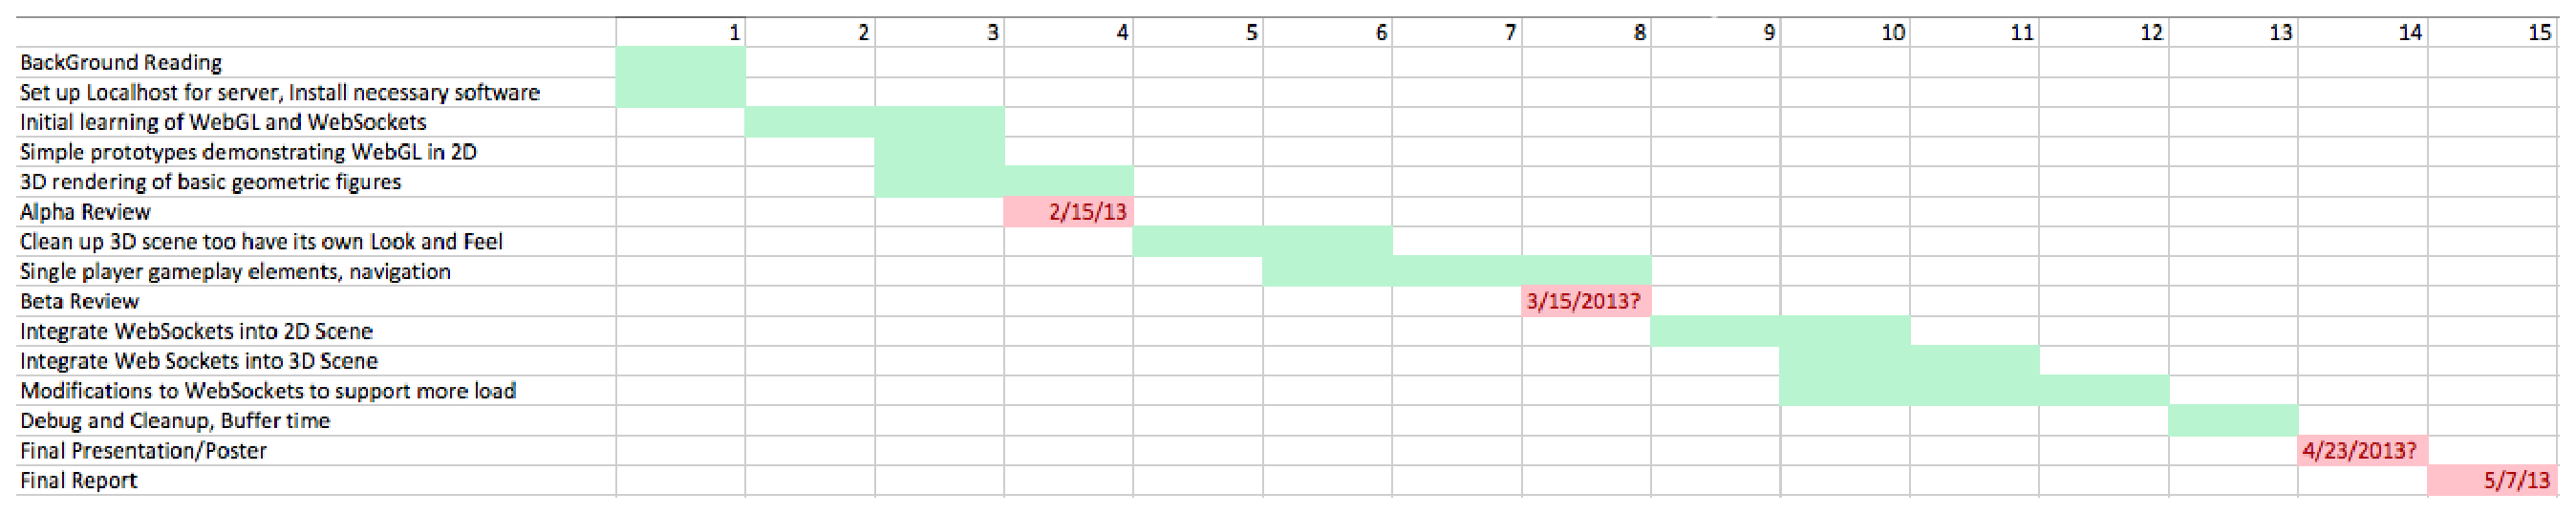
\includegraphics[width=7.5in]{chen_gianni_gantt.eps}
\caption{Gantt Chart Tentative Schedule}
\end{figure*}

\end{document}
